\documentclass[11pt, a4paper]{article}

% --- Sprache und Enkodierung ---
\usepackage[utf8]{inputenc}
\usepackage[T1]{fontenc}
\usepackage[ngerman]{babel}

% --- Layout und Ränder ---
\usepackage{geometry}
\geometry{
    a4paper,
    left=25mm,
    right=25mm,
    top=25mm,
    bottom=25mm,
    headheight=14pt
}

% --- Typografie & Schriftart ---
\usepackage{microtype}
\usepackage{lmodern}
\renewcommand{\familydefault}{\sfdefault}

% --- Grafiken ---
\usepackage{graphicx}
\usepackage{float}

% --- Hyperlinks ---
\usepackage{hyperref}
\hypersetup{
    colorlinks=true,
    linkcolor=blue,
    urlcolor=blue
}

% --- Kopf- und Fußzeilen ---
\usepackage{fancyhdr}
\pagestyle{fancy}
\fancyhf{}
\fancyhead[L]{\textsl{\leftmark}}
\fancyhead[R]{\textsl{Good Knight VR Game}}
\fancyfoot[C]{\thepage}
\renewcommand{\headrulewidth}{0.4pt}
\renewcommand{\footrulewidth}{0.0pt}

\title{Good Knight VR Game\\ \large Dokumentation}
\author{Hikmet Gözaydin 85987}
\date{\today}
\begin{document}

\maketitle
\begin{center}
    \vspace{2cm}
    
\includegraphics[width=0.4\textwidth]{Images/image.png}
\end{center}
\newpage

\tableofcontents
\newpage

\section{Grundidee}
\subsection{Inspiration}
Die Inspiration für dieses Projekt kam, nachdem ich die Serie \textit{A Knight of the Seven Kingdoms} gesehen habe. Die packenden Ritterturniere und Lanzenkämpfe haben mich fasziniert und auf die Idee gebracht, wie spannend ein solches Lanzenkampfspiel in Virtual Reality (VR) wäre. Der Spieltitel \textbf{Good Knight} ist dabei eine direkte Anspielung auf ein Zitat von Prinz Baelor Targaryen: \textit{„I need good men, Ser Duncan“}. Am Ende der Duelle steht man vor der Wahl: Entweder beweist man sich als wahrer Ritter (\textit{„good knight“}) – oder es heißt für einen ganz schnell gute Nacht (\textit{„good night“}).


\subsection{Erster Plan}
Ursprünglich war das Konzept für das Spiel wesentlich umfangreicher gedacht. Ich hatte mir unter anderem Duelle zu Fuß, einen Mehrspielermodus (Multiplayer) sowie ein noch intensiveres Kampfgefühl vorgestellt. Da ich jedoch noch nicht viel Erfahrung in der Spieleentwicklung hatte, habe ich den Aufwand und die Komplexität dieser Features unterschätzt.

Aus diesem Grund habe ich mich letztendlich auf den Kern fokussiert: Ein rundenbasiertes Lanzenkampf-Duell hoch zu Ross zwischen dem Ritter und seinem Gegner.

\newpage
\section{Entwicklung}
\subsection{Das Pferd und der Ritter}
In der ersten Entwicklungsphase lag der Fokus darauf, die beiden Hauptelemente des Spiels (den Ritter und das Pferd) funktional miteinander zu verbinden. Um ein solides Fundament zu schaffen, wurden 3D-Modelle und Assets aus externen Quellen bezogen: Die 3D-Modelle des Ritters und des Pferdes stammen von Sketchfab sowie dem Unity Asset Store, während die grundlegenden Charakteranimationen über Adobe Mixamo generiert wurden. 

Da es sich bei \textit{Good Knight} jedoch um ein Virtual-Reality-Spiel (VR) handelt, konnten diese Ressourcen nicht einfach unverändert übernommen werden. Ein zentrales Element in VR ist die freie Bewegung der Hände über die physischen Controller. Daraus ergab sich die Notwendigkeit, den virtuellen Körper des Ritters dynamisch an die realen Bewegungen des Spielers anzupassen. Um dies zu realisieren, wurde ein System für inverse Kinematik (IK) integriert. Dieses sorgt dafür, dass sich die virtuellen Arme und Gelenke des Ritters anatomisch korrekt beugen und strecken, wenn der Spieler seine Controller bewegt, und dass der restliche Körper (wie Oberkörper und Schultern) diesen Bewegungen auf natürliche Weise folgt.

Eine weitere große Herausforderung lag in der Interaktion zwischen Ritter und Pferd. Standard-Animationen sind meist für stehende oder auf ebenem Boden gehende Charaktere ausgelegt. Für das Reiten mussten die Mixamo-Animationen daher stark angepasst und modifiziert werden. Es war notwendig, die Sitzposition im Sattel manuell zu kalibrieren und die Animationen so anzupassen, dass der Körper des Ritters auf die rhythmischen Bewegungen des Pferdes reagiert. Nur so konnte ein glaubwürdiges und immersives Gefühl des Reitens erzeugt werden, ohne dass die Spielfigur unnatürlich starr auf dem Pferderücken wirkt.


\subsection{Skripte}
Für das Spiel wurden insgesamt 13 C\#-Skripte entwickelt, die in verschiedene funktionale Bereiche unterteilt sind. Die Skripte greifen nahtlos ineinander, um den Ablauf des VR-Lanzenkampfs zu steuern.

\subsubsection{Spielsteuerung und Benutzeroberfläche (Game Management \& UI)}

\noindent
\begin{minipage}[c]{0.45\textwidth}
    \centering
    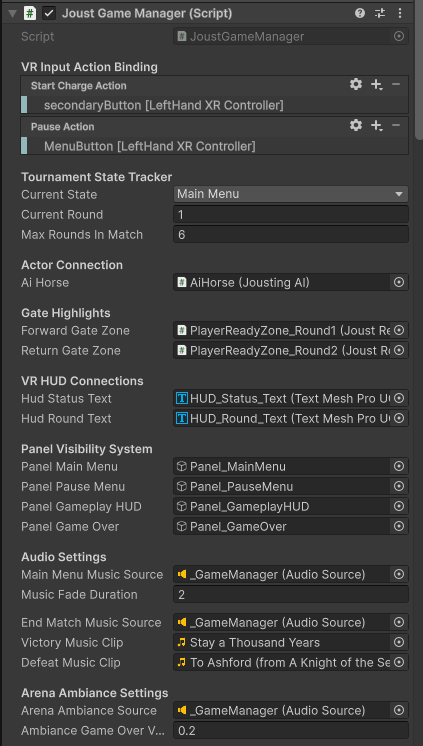
\includegraphics[width=\textwidth]{Images/GameManager.png}
\end{minipage}
\hfill
\begin{minipage}[c]{0.50\textwidth}
    \paragraph{JoustGameManager.cs}
    Die zentrale Zustandsmaschine des Spiels, die den gesamten Spielablauf über sieben Zustände regelt (\textit{MainMenu, BeforeCharge, Countdown, Charging, Resetting, Paused, GameOver}). Sie steuert die Start-Sicherheitsverzögerung, deaktiviert die VR-Fortbewegung bei Rundenbeginn, um ein Herumlaufen zu verhindern, und kontrolliert die Sichtbarkeit der VR-Menüs (Hauptmenü, Pause, HUD, Game Over). Beim Pausieren setzt das Skript \texttt{Physics.autoSimulation = false}, statt die Zeitskalierung einzufrieren. Dadurch bleibt das UI-Raycasting für VR-Interaktionen voll funktionsfähig. Nach der sechsten Runde wertet das Skript die Lebenspunkte aus und entscheidet über Sieg, Niederlage oder Unentschieden. Zudem steuert es die Audio-Fade-Effekte der Musik und der Arena-Atmosphäre.
\end{minipage}
\vspace{0.6cm}

\noindent
\begin{minipage}[c]{0.45\textwidth}
    \centering
    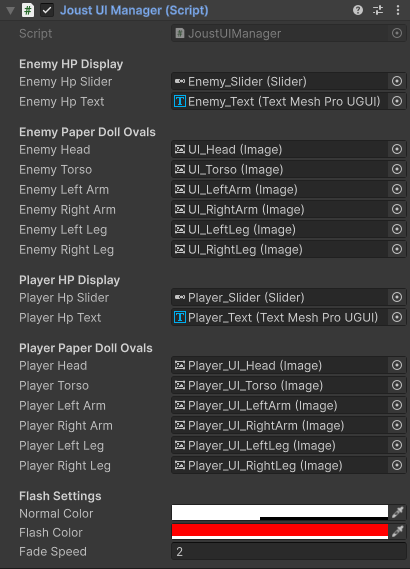
\includegraphics[width=\textwidth]{Images/JoustUiManager.png}
\end{minipage}
\hfill
\begin{minipage}[c]{0.50\textwidth}
    \paragraph{JoustUIManager.cs}
    Steuert das diegetische (in der Spielwelt platzierte) VR-HUD. Es aktualisiert die Lebensbalken und Rundenzähler. Zudem enthält es ein visuelles Schadensmodell des Körpers („Paper Doll“), bei dem getroffene Zonen (Kopf, Torso, Arme, Beine) bei einem Treffer aufleuchten und anschließend weich ausblenden.
\end{minipage}
\vspace{0.6cm}


\subsubsection{Physik, Kampf und Schadensberechnung (Physics, Combat \& Damage)}

\noindent
\begin{minipage}[c]{0.45\textwidth}
    \centering
    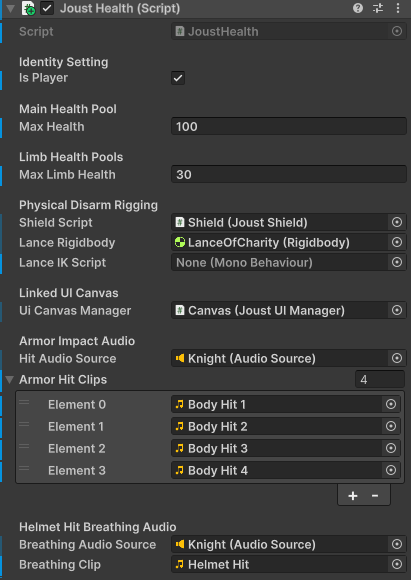
\includegraphics[width=\textwidth]{Images/JoustHealth.png}
\end{minipage}
\hfill
\begin{minipage}[c]{0.50\textwidth}
    \paragraph{JoustHealth.cs}
    Regelt die Lebenspunkte und Trefferzonen von Spieler und KI. Neben dem Hauptpool (100 HP) gibt es separate Arm-Lebenspunkte (je 30 HP). Fällt die Gesundheit des Schildarms (links) auf Null, wird der Schild fallengelassen. Bei Zerstörung des Waffenarms (rechts) wird die Lanze physikalisch gelöst, fallengelassen und die Runde beendet. Das Skript steuert zudem metallische Rüstungtreffersounds und einen Atem-Effekt bei Kopftreffern des Spielers.
\end{minipage}
\vspace{0.6cm}

\noindent
\paragraph{JoustHitbox.cs}
Wird auf die einzelnen Glieder des Skeletts gelegt, um eintreffende Lanzenstöße präzise zu lokalisieren (Kopf, Torso, Arme, Beine). Das Skript berechnet den Schaden anhand eines Multiplikators der jeweiligen Trefferzone und leitet diesen an das übergeordnete \texttt{JoustHealth}-Skript weiter.
\begin{center}
    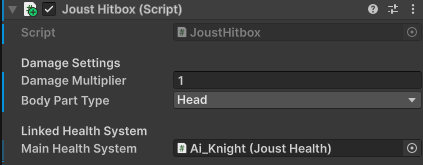
\includegraphics[width=0.4\textwidth]{Images/JoustHitbox.png}
\end{center}
\vspace{0.6cm}

\noindent
\paragraph{JoustLance.cs}
Verwaltet die physikalischen Triggereigenschaften und Kollisionen der Lanzen. Ein eingebautes Verriegelungssystem (Single-Strike Lock) sorgt dafür, dass pro Durchgang nur ein einziger Treffer registriert werden kann, um fehlerhafte Mehrfachtreffer beim Vorbeigaloppieren zu verhindern.
\begin{center}
    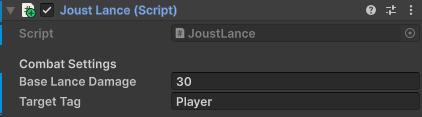
\includegraphics[width=0.4\textwidth]{Images/JoustLance.png}
\end{center}
\vspace{0.6cm}

\noindent
\paragraph{PlayerLance.cs}
Liest über den Rigidbody des Spielerpferdes die aktuelle Galoppgeschwindigkeit aus (\texttt{linearVelocity.magnitude}) und stellt diese über die Methode \texttt{GetStrikeSpeed()} öffentlich zur Verfügung, um den Schaden oder ein Zersplittern der Lanze geschwindigkeitsabhängig zu berechnen.
\vspace{0.6cm}

\noindent
\paragraph{JoustShield.cs}
Ermöglicht das Blocken gegnerischer Angriffe. Bei einem erfolgreichen Block oder bei kritischem Schaden am linken Arm wird der Schild physikalisch vom Ritter gelöst und fällt durch Schwerkraft zu Boden (\texttt{isKinematic = false}, \texttt{useGravity = true}).
\begin{center}
    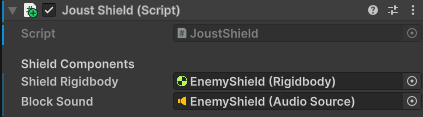
\includegraphics[width=0.4\textwidth]{Images/JoustShield.png}
\end{center}
\vspace{0.6cm}

\subsubsection{Bewegungsmechaniken für Spieler und KI (Player \& AI Movement)}

\noindent
\begin{minipage}[c]{0.45\textwidth}
    \centering
    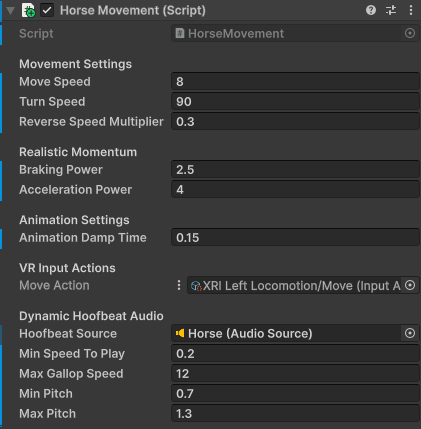
\includegraphics[width=\textwidth]{Images/HorseMovement.png}
\end{minipage}
\hfill
\begin{minipage}[c]{0.50\textwidth}
    \paragraph{HorseMovement.cs}
    Simuliert das Reitverhalten des Spielerpferdes. Es implementiert eine realistische Trägheit mit Beschleunigungs- und Bremskurven und begrenzt die Rückwärtsgeschwindigkeit auf 30\% der Vorwärtsgeschwindigkeit. Außerdem steuert es die Hufgeräusche, deren Lautstärke und Tonhöhe sich dynamisch an die aktuelle Geschwindigkeit des Rigidbodys anpassen.
\end{minipage}
\vspace{0.6cm}

\noindent
\begin{minipage}[c]{0.45\textwidth}
    \centering
    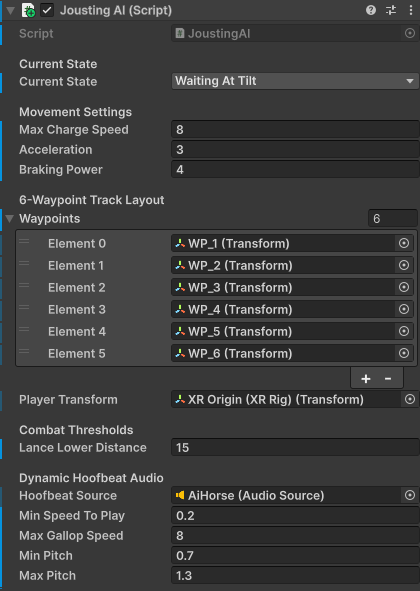
\includegraphics[width=\textwidth]{Images/JoustingAI.png}
\end{minipage}
\hfill
\begin{minipage}[c]{0.50\textwidth}
    \paragraph{JoustingAI.cs}
    Steuert die Bewegung des KI-Gegners entlang eines vordefinierten Pfads aus 6 Wegpunkten (\textit{WP\_1} bis \textit{WP\_3} für ungerade Runden, \textit{WP\_4} bis \textit{WP\_6} für gerade Runden). Ab einer Distanz von 15 Metern zum Spieler signalisiert es dem Animator, die Lanze zu senken. Das Skript berechnet ebenfalls Hufgeräusche, die über 3D-Audio räumlich simuliert werden.
\end{minipage}
\vspace{0.6cm}

\subsubsection{VR-Kameraführung und Kalibrierung (VR Camera \& Calibration)}

\noindent
\begin{minipage}[c]{0.45\textwidth}
    \centering
    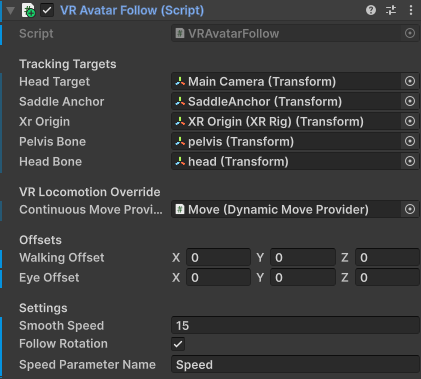
\includegraphics[width=\textwidth]{Images/VRAvatarFollow.png}
\end{minipage}
\hfill
\begin{minipage}[c]{0.50\textwidth}
    \paragraph{VRAvatarFollow.cs}
    Löst die Probleme von Kamera-Drift und Clipping in Virtual Reality. Zu Fuß folgt der Avatar der VR-Brille per LERP. Sobald der Spieler reitet, wird die freie Bewegung deaktiviert und das Becken direkt an den Sattel gekoppelt (\texttt{FixedUpdate}). Die Kamera wird fest im Helm-Mesh positioniert, um zu verhindern, dass der Spieler durch seinen eigenen Körper hindurchsieht.
\end{minipage}
\vspace{0.6cm}

\noindent
\paragraph{VRHeightDebugger.cs}
Ein Diagnosewerkzeug, das 1,0 Sekunden nach dem Szenenstart (sobald das Tracking initialisiert ist) die Höhe der VR-Brille relativ zum Boden überprüft. Es gibt Warnungen in der Konsole aus, falls das Tracking fehlerhaft ist (z. B. wenn die Kamerahöhe auf dem Boden liegt).
\vspace{0.6cm}

\noindent
\paragraph{JoustReadyZone.cs}
Überwacht die Startbereiche der Lanzenbahnen. Das Skript erkennt, ob sich der Spieler im Gatter befindet, steuert die leuchtenden visuellen Markierungsringe und gibt das Signal für den Countdown an den \texttt{JoustGameManager} frei.
\begin{center}
    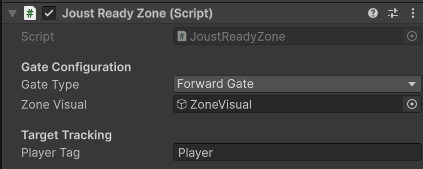
\includegraphics[width=0.4\textwidth]{Images/JoustReadyZone.png}
\end{center}
\vspace{0.6cm}

\subsubsection{KI-Lanzensteuerung über Inverse Kinematik (AILanceCombatIK.cs)}

\noindent
\begin{minipage}[c]{0.45\textwidth}
    \centering
    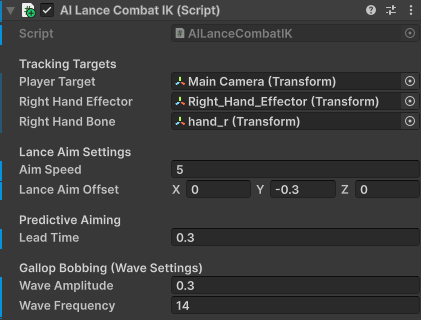
\includegraphics[width=\textwidth]{Images/AILanceCombatIK.png}
\end{minipage}
\hfill
\begin{minipage}[c]{0.50\textwidth}
    \paragraph{AILanceCombatIK.cs}
    Steuert die physikalische Zielausrichtung der gegnerischen Lanze mittels Unity-IK. Im \texttt{LateUpdate} wird der rechte IK-Effektor fest an die Hand des KI-Modells geheftet. Um eine lose Kopplung zu wahren, liest das Skript den aktuellen Zustand der KI via C\#-Reflection aus. Die Verfolgung des Spielers ist nur aktiv, wenn sich die KI in den Zuständen \textit{Charging} oder \textit{LoweringLance} befindet; andernfalls wird die Lanze parallel zur Wirbelsäule des Pferdes geparkt. Beim Zielen berechnet das Skript prädiktiv die Bewegung des Spielers anhand seiner Geschwindigkeit und zielt um eine Vorhaltezeit (\textit{leadTime} = 0,15 Sekunden) voraus. Um den holprigen Galopp zu simulieren, wird der Ausrichtung eine prozedurale Sinuskurve (Sinuswelle mit einstellbarer Frequenz und Amplitude) überlagert. Im Parkmodus werden die Positionsdaten im Hintergrund geräuschlos aktualisiert, um sprunghafte Bewegungen beim Start einer neuen Runde zu vermeiden.
\end{minipage}
\vspace{0.6cm}


\subsection{Sound}
Die auditive Kulisse von \textit{Good Knight} spielt eine entscheidende Rolle für die Immersion in Virtual Reality. Die Soundeffekte und Musikstücke wurden sorgfältig ausgewählt, bei Bedarf mit der Open-Source-Audio-Software \textbf{Audacity} angepasst (z. B. gekürzt, in der Lautstärke kalibriert oder für Looping-Effekte vorbereitet) und an verschiedenen Stellen im Spiel integriert. Die Implementierung umfasst dynamische Fading-Effekte sowie 3D-Kopfkollisions-Audio:


\subsubsection{Musik und Atmosphäre}
\begin{itemize}
    \item \textbf{Hauptmenü-Musik:} \textit{„Main Title / Let the Gods Decide“} von Dan Romer (aus dem Soundtrack zur HBO-Serie \textit{A Knight of the Seven Kingdoms}). Diese läuft in einer Endlosschleife im Hauptmenü. Sobald das Spiel startet, wird sie über das Skript \texttt{JoustGameManager.cs} mittels einer Coroutine (\texttt{FadeOutMusicRoutine}) sanft ausgeblendet.
    
    \item \textbf{Sieg-Musik:} \textit{„Stay a Thousand Years“} von Ramin Djawadi (aus \textit{Game of Thrones} Staffel 8). Sie ertönt in einer Schleife auf dem Game-Over-Bildschirm, wenn der Spieler das Turnier gewinnt (entweder durch Knockout des Gegners oder nach Punkten nach der 6. Runde).
    
    \item \textbf{Niederlage-Musik:} \textit{„To Ashford“} von Dan Romer (aus \textit{A Knight of the Seven Kingdoms}). Sie wird abgespielt, wenn der Spieler vom Pferd gestoßen wird oder nach Punkten verliert.
    
    \item \textbf{Arena-Hintergrundgeräusche (Ambience):} \textit{„Welcome to the Arena - RPG Ambience“} (von YouTube). Diese Tonspur läuft während der gesamten Spielphase und simuliert das Publikum in der Arena. Bei einem Match-Ende (Game Over) wird die Lautstärke über die Coroutine \texttt{FadeAmbianceToGameOverRoutine} auf $20\%$ gedimmt, um die Sieges- oder Niederlagenmusik klar hervorzuheben.
\end{itemize}

\subsubsection{Gameplay- und Kollisionsgeräusche}
\begin{itemize}
    \item \textbf{Pferdegalopp (Hoofbeats):} \textit{„Running Horse with a Rider“} von \textit{sonically\_sound} (Freesound ID 645465). Dieses Hufgeräusch wird von \texttt{HorseMovement.cs} (Spieler) und \texttt{JoustingAI.cs} (KI) genutzt. Die Lautstärke und die Tonhöhe (Pitch) werden in Echtzeit proportional zur Rigidbody-Geschwindigkeit angepasst ($0.7$ bis $1.3$ Pitch). Bleibt das Pferd stehen, stoppt das Geräusch mit einem Fade-out. Bei der KI wird das Geräusch mit vollem räumlichen 3D-Panning abgespielt, wodurch das herannahende Pferd akustisch geortet werden kann.
    
    \item \textbf{Schildtreffer (Shield Hit):} \textit{„Plate Armor - Hit 4“} von \textit{sgossner} (Freesound ID 209401). Dieses Geräusch wird abgespielt, wenn die Lanze erfolgreich auf dem gegnerischen Schild aufschlägt.
    
    \item \textbf{Körpertreffer (Body Hit):} Ein Rüstungstreffer-Sound aus dem YouTube-Video \textit{srkI6Y6xgeU} (wird in \texttt{JoustHealth.cs} als Teil des \texttt{armorHitClips}-Arrays aufgerufen). Bei einem Treffer an Kopf oder Torso wird zufällig einer von vier verschiedenen Rüstungskollision-Sounds abgespielt.
    
    \item \textbf{Gehirnerschütterung/Schweres Atmen (Helmet Hit Breathing):} \textit{„knight's breath in his helmet“} von \textit{graneodin\_6} (Freesound ID 747772). Wenn der Spieler einen direkten Treffer an den Helm (Kopf) erleidet, triggert das Skript \texttt{JoustHealth.cs} ein 2D-Atemgeräusch, um das Gefühl eines schweren Kopftraumas oder einer Gehirnerschütterung im Helm akustisch zu simulieren.
\end{itemize}

\newpage
\section{Spielmechaniken}
Dieses Kapitel beschreibt die zentralen Spielmechaniken von \textit{Good Knight}, aufgeteilt in vier Kernbereiche. Die Mechaniken wurden auf Basis der physikalischen Gesetze und VR-Anforderungen entwickelt, um ein immersives und anspruchsvolles Gameplay zu garantieren.

\subsection{Turnierstruktur und Rundenablauf (Das Schiedsrichter-System)}
Der gesamte Ablauf eines Turniers wird von einer zentralen Zustandsmaschine (\texttt{JoustGameManager.cs}) gesteuert, die sieben diskrete Spielzustände verwaltet (\textit{MainMenu, BeforeCharge, Countdown, Charging, Resetting, Paused, GameOver}):
\begin{itemize}
    \item \textbf{Das 6-Durchgänge-Format:} Ein Match ist strikt auf maximal 6 Durchgänge (Pässe) limitiert.
    \item \textbf{Abwechselnde Bahnen:} Um den authentischen Regeln eines Tjosts zu entsprechen, wechseln die Durchgänge die Richtung. In ungeraden Runden (1, 3, 5) reiten die Kontrahenten in der Vorwärtsbahn, in geraden Runden (2, 4, 6) in der Rückwärtsbahn.
    \item \textbf{Startgatter-Mechanik:} Vor dem Start eines Durchgangs muss der Spieler sein Pferd in den leuchtenden Markierungsring des jeweiligen Startgatters steuern. Sobald er stillsteht und Bereitschaft signalisiert, startet der 3-Sekunden-Countdown.
    \item \textbf{Vorzeitiges Match-Ende:} Ein Match endet sofort vorzeitig, wenn ein Ritter unhorsed wird (seine Hauptgesundheit auf Null fällt) oder sein Waffenarm verkrüppelt wird (Entwaffnung).
    \item \textbf{Entscheidung nach Punkten:} Überleben beide Ritter alle 6 Durchgänge, vergleicht der Schiedsrichter die verbleibenden Lebenspunkte. Der Ritter mit der höheren verbleibenden Gesundheit gewinnt das Turnier. Sind die Lebenspunkte identisch, endet das Match unentschieden.
\end{itemize}

\subsection{Fortbewegung des Pferdes und Wegpunkt-Navigation}
Die Steuerung und Bewegung des Pferdes sind so konzipiert, dass sich das Reiten eines schweren Schlachtrosses träge, schwer und physikalisch glaubwürdig anfühlt:
\begin{itemize}
    \item \textbf{Realistische Trägheit:} Sowohl der Spieler als auch die KI unterliegen berechneten Beschleunigungs- und Bremsphasen. Das Pferd reagiert verzögert wie ein schweres Tier und nicht wie eine Spielfigur im Arcade-Stil.
    \item \textbf{Rückwärts-Geschwindigkeitsbegrenzer:} Die Geschwindigkeit beim Rückwärtsreiten ist auf $30\%$ der Vorwärtsgeschwindigkeit limitiert. Dies verhindert hektische und unrealistische Bewegungen beim Positionieren am Startgatter.
    \item \textbf{KI-Wegpunkt-Navigation:} Die KI nutzt ein vordefiniertes Wegpunktraster aus 6 Punkten. Sie reitet die zugewiesene Bahn (Startgatter $\rightarrow$ Mittelpunkt $\rightarrow$ Endgatter) ab und führt nach jedem Durchgang einen seitlichen Spurwechsel durch, um sich für die Gegenrichtung zu positionieren.
    \item \textbf{VR-Sattelkopplung:} Um Bewegungsübelkeit (Motion Sickness) zu vermeiden und Kameraverzögerungen zu eliminieren, wird die Position und Rotation des Spielers im Sattel starr mit dem Pferd synchronisiert (\texttt{FixedUpdate}). Die freie Fortbewegung zu Fuß per Controller-Joystick wird im Sattel deaktiviert; stattdessen dient der linke Joystick nun der Steuerung und Beschleunigung des Pferdes.
\end{itemize}

\subsection{Kampf, Zielen und Inverse Kinematik (IK)}
Der Kampf basiert auf präzisem räumlichen Zielen und gutem Timing beim Ausweichen oder Blocken:
\begin{itemize}
    \item \textbf{Prädiktives Zielen der KI:} Die KI zielt nicht stumpf auf die aktuelle Position des Spielers. Sie berechnet die Echtzeit-Geschwindigkeit des Spielers und zielt um eine Vorhaltezeit (\textit{leadTime} = 0,15 Sekunden) voraus. Der Spieler wird dadurch gezwungen, aktiv auszuweichen oder den Schild hochzureißen.
    \item \textbf{Prozedurales Wippen:} Um den Ritt auf einem galoppierenden Pferd zu simulieren, wird der Lanzenführung der KI eine mathematische Sinuswelle überlagert. Dies erzeugt eine natürliche Ungenauigkeit beim Zielen der KI.
    \item \textbf{Kontextabhängiges Absenken der gegnerischen Lanze (nur KI):} Um Clipping-Fehler beim Reiten zu vermeiden, hält die KI ihre Lanze in der Vorbereitung aufrecht (geparkt). Erst wenn sich die Kontrahenten auf weniger als 15 Meter genähert haben, senkt die KI ihre Lanze automatisch in die Zielposition ab. Der Spieler hingegen kontrolliert die Ausrichtung seiner Lanze jederzeit manuell über den VR-Controller.
    \item \textbf{Schild-Schadensminderung:} Der Spieler muss den Schild an seinem linken Arm manuell so positionieren, dass er die eintreffende gegnerische Lanze abfängt. Frontale Treffer auf dem Schild verhindern den Schaden, führen jedoch nach dem Block zum Verlust des Schildes.
\end{itemize}

\subsection{Schadensberechnung und Entwaffnungssystem}
Das Schadensmodell ist modular aufgebaut und teilt den Körper in anatomische Zonen mit direkten spielmechanischen Konsequenzen:
\begin{itemize}
    \item \textbf{Einzeltreffer-Verriegelung:} Um Mehrfachtreffer durch Kollisions-Exploits während eines Vorbeigaloppierens zu verhindern, verriegeln sich die Lanzen nach dem ersten registrierten Treffer für den Rest des Durchgangs.
    \item \textbf{Modulare Anatomie:} Jeder Charakter besitzt eine Hauptgesundheit von 100 HP sowie separate Gliedmaßen-Lebenspunkte von je 30 HP für den linken und rechten Arm.
    \item \textbf{Verkrüppelung des Schildarms:} Sinkt die Gesundheit des linken Arms auf Null, bricht dieser spielmechanisch. Der Schild wird augenblicklich fallengelassen und ist für den Rest des Turniers verloren.
    \item \textbf{Verkrüppelung des Waffenarms:} Fällt die Gesundheit des rechten Arms auf Null, wird der Ritter entwaffnet. Die Lanze fällt zu Boden, was das sofortige Ende der Runde (und die Niederlage bzw. den Sieg) zur Folge hat.
\end{itemize}

\newpage
\section{Herausforderungen}
Im Laufe der Entwicklung von \textit{Good Knight} mussten mehrere technische und gestalterische Hürden überwunden werden. Die drei größten Herausforderungen waren:

\begin{enumerate}
    \item \textbf{VR-Übelkeit (Motion Sickness):} 
    Die Reduzierung der Bewegungskrankheit (Motion Sickness) bei dem wellenartigen Galopp war eine große Herausforderung. Durch das Deaktivieren der Joystick-Steuerung und das starre Festkoppeln der Kamera an das Pferd in \texttt{FixedUpdate} konnten Verzögerungen minimiert werden. Dennoch lässt sich eine gewisse Übelkeit bei längeren Spielsessions aufgrund der ständigen Wippbewegung und hohen Geschwindigkeit auf Dauer leider nicht vollständig verhindern.
    
    \item \textbf{Kollisionen \& Physik:} 
    Die Physikberechnung bei hohen Geschwindigkeiten (wenn zwei galoppierende Pferde aufeinander treffen) stellte sich als äußerst fehleranfällig heraus. Ohne Optimierung kam es häufig dazu, dass Lanzen die Hitboxen durchdrangen, ohne Schaden zu verursachen, oder durch anhaltenden Kontakt mehrere Treffer im selben Durchgang auslösten. Dies wurde durch präzise Trigger-Abfragen und die Implementierung einer Einzeltreffer-Verriegelung (\texttt{hasHitSomethingThisPass} in \texttt{JoustLance.cs}) gelöst. Zudem wurde die Vektorberechnung verfeinert, damit Schilde und Rüstungsplatten eingehende Lanzenstöße physikalisch korrekt abwehren oder ablenken.
    
    \item \textbf{Animationen \& IK (Inverse Kinematik):} 
    Die Anpassung von vorgefertigten Mixamo-Animationen an die Sitzhaltung auf einem 3D-Pferdemodell war ein komplexer manueller Prozess. Da Standardanimationen für stehende Charaktere gedacht sind, mussten diese für das Reiten umgebogen und gestreckt werden. Die größte Schwierigkeit lag in der Implementierung der inversen Kinematik (IK): Es galt sicherzustellen, dass die Arme des Ritters den VR-Controllern des Spielers flüssig folgen, sich dabei aber nicht unnatürlich verdrehen, und dass der KI-Gegner mithilfe von mathematischem Vorhalten prädiktiv nach der Spielerposition zielt.
\end{enumerate}

\newpage
\section{Assets}
In diesem Kapitel werden alle extern bezogenen Assets (3D-Modelle, Umgebungen, Musikstücke und Soundeffekte) dokumentiert und verlinkt.

\subsection{3D-Modelle und Umgebungs-Packs}
Für die visuelle Gestaltung der Charaktere und der Tjost-Arena wurden folgende 3D-Modelle verwendet:

\begin{description}
    \item[Ritter-Charaktermodell:] \textit{Modular Fantasy knight character} von Anton Puzanov (Unity Asset Store). 
    Ein vollständig modular aufgebautes 3D-Modell eines Ritters in Plattenrüstung, das für die Spielfigur und den KI-Gegner verwendet wird. \\
    Link: \href{https://assetstore.unity.com/packages/3d/characters/humanoids/fantasy/modular-fantasy-knight-character-276754}{Unity Asset Store}
    
    \item[Pferdemodell:] \textit{Horse} von Henry S (@henry\_7) (Sketchfab).
    Ein detailliertes 3D-Modell eines Pferdes, welches die Grundlage für das Reitpferd des Spielers und des Gegners bildet. \\
    Link: \href{https://sketchfab.com/3d-models/horse-a6f860e43e364619bccb174a1ac7d0c9}{Sketchfab}
    
    \item[Holzzäune und Holzschranken:] \textit{Medieval Pack - Wood set \#1} von Théo Lerbeil (Fab.com).
    Ein Set aus mittelalterlichen Holzobjekten, das für die Abgrenzung der Jousting-Lanzenbahn (den sogenannten „Tilt“) verwendet wird. \\
    Link: \href{https://www.fab.com/listings/cd1e2cdd-f399-4a68-a7f7-e842e2e26852}{Fab.com}
    
    \item[Turnierarena:] \textit{Old battle arena} von Rixael (Sketchfab).
    Das 3D-Modell einer alten Kampfarena, das als Hauptkulisse (Tjost-Platz) dient. \\
    Link: \href{https://sketchfab.com/3d-models/old-battle-arena-9dad465609334aef8f1d99c37a30c940}{Sketchfab}
    
    \item[Ruinenumgebung:] \textit{[SCANS] Ruined Crypt} von Scans Factory (Fab.com).
    Ein photogrammetriebasiertes Asset-Pack mit alten Ruinen- und Waldobjekten zur stimmungsvollen Dekoration des restlichen Arenabereichs. \\
    Link: \href{https://www.fab.com/listings/ea85f730-1f39-4b15-8a69-60975d3b39a7}{Fab.com}
    
    \item[Lanzenmodell:] \textit{Lance Of Charity} von IZ (@I.Z.) (Sketchfab).
    Das 3D-Modell der ritterlichen Turnierlanze, mit der beide Kontrahenten ausgestattet sind. \\
    Link: \href{https://sketchfab.com/3d-models/lance-of-charity-e2b7e77ca95f468b99d7941ad5bf80f1}{Sketchfab}
\end{description}

\subsection{Musikstücke und Soundeffekte}
Für die akustische Untermalung wurden die folgenden Sound-Assets verwendet, die teilweise in Audacity nachbearbeitet wurden:

\begin{description}
    \item[Hauptmenü-Musik:] \textit{„Main Title / Let the Gods Decide“} von Dan Romer. \\
    Link: \href{https://music.youtube.com/watch?v=AfjQ9JGxHNg}{YouTube Music}
    
    \item[Sieg-Musik:] \textit{„Stay a Thousand Years“} von Ramin Djawadi. \\
    Link: \href{https://music.youtube.com/watch?v=MP7zZ_ZFUBo}{YouTube Music}
    
    \item[Niederlage-Musik:] \textit{„To Ashford“} von Dan Romer. \\
    Link: \href{https://music.youtube.com/watch?v=a1HiKCwwTzo}{YouTube Music}
    
    \item[Arena-Ambiente:] \textit{„Welcome to the Arena - RPG Ambience“}. \\
    Link: \href{https://www.youtube.com/watch?v=pUypls1WgCg}{YouTube}
    
    \item[Pferdegalopp (Hoofbeats):] \textit{„Running Horse with a Rider“} von \textit{sonically\_sound} (Freesound ID 645465). \\
    Link: \href{https://freesound.org/people/sonically_sound/sounds/645465/}{Freesound}
    
    \item[Schildtreffer (Shield Hit):] \textit{„Plate Armor - Hit 4“} von \textit{sgossner} (Freesound ID 209401). \\
    Link: \href{https://freesound.org/people/sgossner/sounds/209401/}{Freesound}
    
    \item[Körpertreffer (Body Hit):] \textit{Plate Armor Body Hit}. \\
    Link: \href{https://www.youtube.com/watch?v=srkI6Y6xgeU}{YouTube}
    
    \item[Gehirnerschütterung/Atmen:] \textit{„knight's breath in his helmet“} von \textit{graneodin\_6} (Freesound ID 747772). \\
    Link: \href{https://freesound.org/people/graneodin_6/sounds/747772/}{Freesound}
\end{description}


\end{document}
